It is essential for the users of the application to have accounts. It enables user interaction and many of the features that are desired in a marketplace application. User's expect their actions and settings persisted across platforms. However, they expect some privacy. Other users should not be able to see their private details. This all leads to the need of having authentication methods in the application. The way it is handled in the application is by allowing three authentication methods: Facebook, Google and email address. Going forward we will only look at email address, as that is GulOgGratis own implementation. 

When you create an account the default information is entered and you press create. Looking at the network traffic some validation of various fields are performed. An example is verifying the email is not in use. The application then sends the information to the server, an account is created, the application performs a login request and the server returns tokens. However the email was never verified. The server returns a JWT (JSON Web Token) and another token consisting of forty characters. A decoded JWT can be seen on Figure \ref{fig:jwt_decoded}. The header indicates that the token is signed using HMAC-SHA256 and the payload contains some user information. It is unclear looking at the network traffic and the source code what the JWT is used for. Meanwhile the other undefined token is stored locally and used in every HTTP request.  

\begin{figure}[htbp]
    \centering
    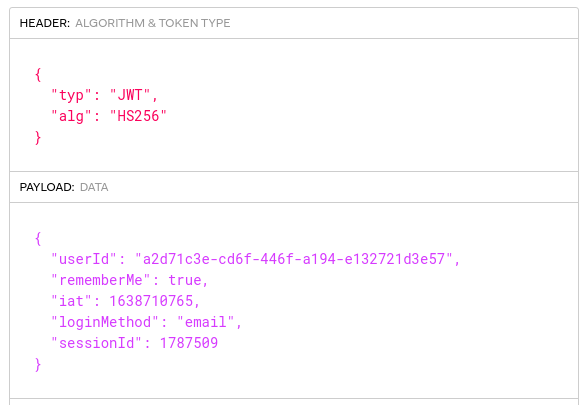
\includegraphics[width=0.7\columnwidth]{../dynamic-analysis/pictures/jwt_decoded.png}
    \caption{Decoded JSON Web Token}
    \label{fig:jwt_decoded}
\end{figure}

Having created the account you can sign in using your email and password. The application then calls the api with a login action and the tokens are returned. The user is then authenticated and ready to use them for further actions. The used token is persisted in the application's local directory. When the user then signs out no network traffic is detected. However looking at the code it is seen that the token, user address and user id are removed from local storage.      

The password used for authenticating is quite unrestricted. The only requirements are that they need to be at least eight signs and a combination of numbers and letters. Additionally, when changing the password it is allowed to change to one that has already been used, and changing it to the exact same. Resetting the password results in no received email even though a request is detected. Trying to perform the reset on the web site results in an instantaneous received email. Inspecting that traffic it is interesting to see that it utilizes another hostname and the request is completely different. This might indicate that the API the mobile application utilizes is becoming obsolete.     

In the system it is possible to validate your account with NemID. This ensures you are the person who you indicate you are. This is a safety for others interacting with you. The validation can only happen through the web site. 

